\documentclass[11pt,a4paper]{article}

% --- Paquetes Esenciales para Overleaf ---
\usepackage[utf8]{inputenc}
\usepackage[T1]{fontenc}
\usepackage[spanish,es-tabla]{babel}
\usepackage[top=2.2cm,bottom=2.2cm,left=2.2cm,right=2.2cm]{geometry}
\usepackage{graphicx}
\usepackage{xcolor}
\usepackage{fancyhdr}
\usepackage{titlesec}
\usepackage{tcolorbox}
\usepackage{listings}
\usepackage{booktabs}
\usepackage{float}
\usepackage{caption}
\usepackage{enumitem}
\usepackage{microtype}
\usepackage{hyperref}

% --- Paleta de Colores Institucionales SENA ---
\definecolor{senaGreen}{HTML}{00A86B}
\definecolor{senaDark}{HTML}{0F172A}
\definecolor{senaLight}{HTML}{ECFDF5}
\definecolor{techBlue}{HTML}{2563EB}
\definecolor{techBlueLight}{HTML}{EFF6FF}
\definecolor{codeBg}{HTML}{0F172A}
\definecolor{codeText}{HTML}{38BDF8}
\definecolor{cardBorder}{HTML}{CBD5E1}
\definecolor{textMuted}{HTML}{64748B}

% --- Configuración de Enlaces Hipertexto ---
\hypersetup{
    colorlinks=true,
    linkcolor=techBlue,
    filecolor=techBlue,
    urlcolor=senaGreen,
    citecolor=techBlue,
    pdftitle={GA7-220501096-AA1-EV04: Instalación y Configuración de Herramientas de Versionamiento},
    pdfauthor={Karen Yuliana Campo},
    pdfsubject={SENA ADSO Ficha 228118}
}

% --- Configuración de Encabezados y Pies de Página ---
\pagestyle{fancy}
\fancyhf{}
\fancyhead[L]{\small\textbf{\color{senaGreen}SENA ADSO • Ficha 228118} | Guía 7 (AP7)}
\fancyhead[R]{\small\color{textMuted}GA7-220501096-AA1-EV04}
\fancyfoot[L]{\small\color{textMuted}Karen Yuliana Campo • Popayán, Cauca}
\fancyfoot[R]{\small\color{textMuted}Página \thepage}
\renewcommand{\headrulewidth}{0.8pt}
\renewcommand{\footrulewidth}{0.4pt}

% --- Configuración de Títulos de Sección ---
\titleformat{\section}
  {\normalfont\Large\bfseries\color{senaDark}}{\thesection}{1em}{}[\titlerule]
\titleformat{\subsection}
  {\normalfont\large\bfseries\color{techBlue}}{\thesubsection}{1em}{}
\titleformat{\subsubsection}
  {\normalfont\normalsize\bfseries\color{senaGreen}}{\thesubsubsection}{1em}{}

% --- Cajas Estilizadas para Comandos y Pasos ---
\newtcolorbox{stepbox}[2][]{
  colback=white,
  colframe=cardBorder,
  coltitle=senaDark,
  fonttitle=\bfseries,
  title=#2,
  boxrule=1pt,
  arc=3mm,
  left=6pt, right=6pt, top=6pt, bottom=6pt,
  #1
}

\newtcolorbox{cmdbox}[1][]{
  colback=codeBg,
  colframe=senaDark,
  arc=2mm,
  left=8pt, right=8pt, top=6pt, bottom=6pt,
  #1
}

% --- Configuración de Listings para Código ---
\lstset{
  backgroundcolor=\color{codeBg},
  basicstyle=\ttfamily\footnotesize\color{white},
  keywordstyle=\color{codeText}\bfseries,
  commentstyle=\color{textMuted}\itshape,
  stringstyle=\color{senaGreen},
  breaklines=true,
  showstringspaces=false,
  frame=none
}

\begin{document}

% =========================================================================
% PORTADA INSTITUCIONAL FORMAL
% =========================================================================
\begin{titlepage}
    \centering
    \vspace*{0.5cm}
    
    {\Huge\bfseries\color{senaGreen} SERVICIO NACIONAL DE APRENDIZAJE\\[0.2cm] (SENA)\par}
    \vspace{0.4cm}
    {\large\textbf{\color{senaDark} Regional Cauca -- Centro de Comercio y Servicios}\par}
    \vspace{0.2cm}
    {\normalsize Tecnólogo en Análisis y Desarrollo de Software (ADSO) -- Modalidad 100\% Virtual\par}
    \vspace{0.1cm}
    {\normalsize\textbf{Ficha de Caracterización: 228118}\par}
    
    \vspace{1.2cm}
    \rule{\linewidth}{1.5pt}\\[0.4cm]
    {\LARGE\bfseries\color{senaDark} GUÍA DE APRENDIZAJE 7 (AP7)\\[0.25cm]
    \Large INFORME TÉCNICO DE INSTALACIÓN Y CONFIGURACIÓN DE HERRAMIENTAS DE VERSIONAMIENTO (LOCAL / WEB)\\[0.3cm]
    \large\color{techBlue} Evidencia: GA7-220501096-AA1-EV04\par}
    \rule{\linewidth}{1.5pt}
    
    \vspace{1.5cm}
    
    \begin{tcolorbox}[colback=senaLight,colframe=senaGreen,arc=3mm,width=0.92\linewidth]
        \centering
        \textbf{\large Proyecto Formativo:}\\[0.15cm]
        \textit{Sistema de Información y Gestión de Pedidos para ``Pizzería Bella Italia''}\\[0.3cm]
        \textbf{Competencia Técnica:} 220501096 -- Desarrollar la solución de software de acuerdo con el diseño y metodologías de desarrollo\\[0.15cm]
        \textbf{Componente Formativo de Referencia:} Integración continua
    \end{tcolorbox}
    
    \vspace{1.8cm}
    
    \begin{minipage}{0.48\textwidth}
        \flushleft
        \textbf{\color{senaDark} Aprendiz Desarrolladora:}\\
        Karen Yuliana Campo\\
        Ficha: 228118\\
        ADSO 100\% Virtual
    \end{minipage}
    \hfill
    \begin{minipage}{0.48\textwidth}
        \flushright
        \textbf{\color{senaDark} Ubicación y Fecha:}\\
        Popayán, Cauca, Colombia\\
        Noviembre de 2026\\
        Calificación: Lista IE-GA7-220501096-AA1-EV04
    \end{minipage}
    
    \vfill
\end{titlepage}

% =========================================================================
% TABLA DE CONTENIDO
% =========================================================================
\tableofcontents
\newpage

% =========================================================================
% SECCIÓN 1: INTRODUCCIÓN
% =========================================================================
\section{Introducción}

En el ciclo de vida de la ingeniería de software actual, el control de versiones constituye la piedra angular sobre la que se erigen la colaboración en equipo, la integridad de los artefactos de código y los procesos modernos de entrega continua (\textit{Continuous Delivery}). Históricamente, las soluciones centralizadas (\textit{CVS, SVN}) presentaban un punto único de fallo (\textit{Single Point of Failure}); si el servidor central quedaba fuera de servicio o se interrumpía la red, los ingenieros se veían imposibilitados de confirmar cambios, inspeccionar el árbol de versiones o crear ramas de trabajo.

La adopción de \textbf{Git} como sistema de control de versiones distribuido (\textit{DVCS -- Distributed Version Control System}) resolvió esta limitación al proveer a cada estación de trabajo un clon completo del repositorio, incluyendo su base de datos inmutable de objetos (\textit{commits, trees y blobs}). Para materializar una arquitectura de trabajo profesional en el proyecto formativo \textbf{Pizzería Bella Italia}, es imperativo articular de forma sinérgica:
\begin{enumerate}[label=\alph*)]
    \item \textbf{El entorno Git Local:} Instalado en el sistema operativo del desarrollador (Windows 11), permitiendo registrar confirmaciones con latencia casi nula ($<10\,\text{ms}$) y operar en modo totalmente desconectado (\textit{offline}).
    \item \textbf{El entorno Git Remoto (GitHub):} Plataforma en la nube que actúa como repositorio centralizado para respaldo georredundante, revisión de código (\textit{Code Review}) mediante \textit{Pull Requests} y disparador de compuertas automatizadas de aseguramiento de calidad con \textit{GitHub Actions}.
\end{enumerate}

Tomando como base las directrices del componente formativo \textbf{``Integración continua''} de la Guía de Aprendizaje 7, este documento presenta el manual técnico ilustrado, paso a paso, de la instalación de Git para Windows y la apertura y parametrización de la cuenta en GitHub realizada por la aprendiz Karen Yuliana Campo en la ciudad de Popayán, Cauca.

% =========================================================================
% SECCIÓN 2: OBJETIVOS
% =========================================================================
\section{Objetivos}

\subsection{Objetivo General}
Documentar e ilustrar de forma exhaustiva el procedimiento técnico de instalación, parametrización y verificación de la herramienta de control de versiones \textbf{Git local} en entorno Windows, así como el registro y configuración del perfil en la plataforma web \textbf{Git remoto (GitHub)}, fundamentando su articulación en el proyecto de la Pizzería Bella Italia.

\subsection{Objetivos Específicos}
\begin{itemize}[leftmargin=1.5cm]
    \item[1.] Detallar los 19 pasos del asistente de instalación de Git para Windows mediante capturas de pantalla reales, justificando las selecciones técnicas efectuadas (editor predeterminado, nombre de rama inicial \texttt{main}, integración con PATH y conversión de finales de línea).
    \item[2.] Documentar el flujo de registro, verificación de correo y configuración inicial de la cuenta remota en GitHub.
    \item[3.] Establecer los comandos de consola en \textit{Git Bash} para verificar la versión instalada (\texttt{git -{}-version}) y parametrizar las variables de identidad global (\texttt{user.name} y \texttt{user.email}).
    \item[4.] Responder integralmente a cada uno de los criterios exigidos en la lista de chequeo \textbf{IE-GA7-220501096-AA1-EV04} de la Guía 7.
\end{itemize}

\newpage

% =========================================================================
% SECCIÓN 3: INSTALACIÓN DE GIT LOCAL EN WINDOWS (PASO A PASO)
% =========================================================================
\section{Instalación de Git Local en Windows (Paso a Paso con Capturas Reales)}

A continuación se presenta el registro secuencial de la instalación ejecutada en el equipo de desarrollo de la aprendiz en Popayán, utilizando el instalador oficial de 64 bits para Windows:

\subsection{Paso 1: Descarga del Instalador Oficial}
Se ingresa al portal oficial del proyecto (\url{https://git-scm.com/download/win}) y se descarga el instalador independiente para Windows de 64 bits (\textit{Git Standalone Installer}).

\begin{figure}[H]
    \centering
    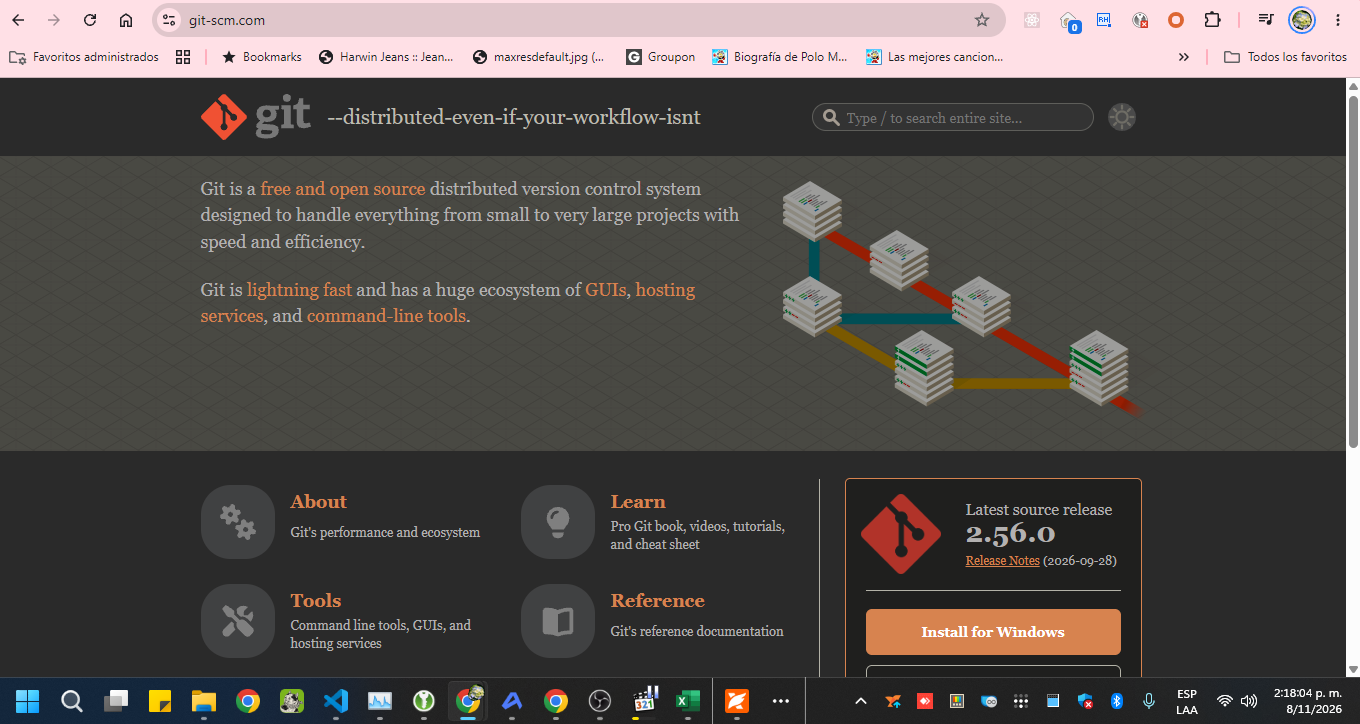
\includegraphics[width=0.88\linewidth]{images/local/paso_01.png}
    \caption{Descarga del instalador de Git para Windows desde el sitio web oficial.}
    \label{fig:local_01}
\end{figure}

\subsection{Paso 2: Información de Licencia de Software (GPLv2)}
Al ejecutar el binario instalador con privilegios de administrador, se visualizan los términos de la licencia \textit{GNU General Public License v2}, garantizando el uso libre, modificación y distribución del software.

\begin{figure}[H]
    \centering
    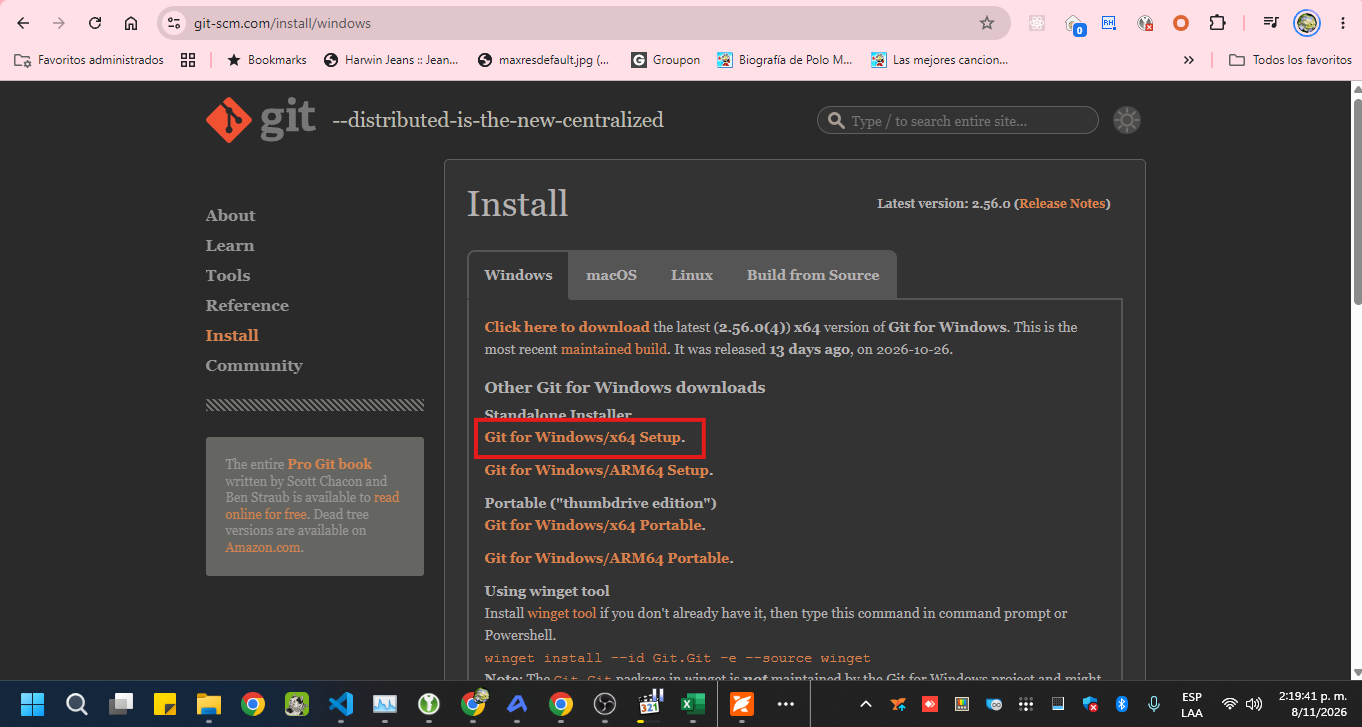
\includegraphics[width=0.85\linewidth]{images/local/paso_02.png}
    \caption{Pantalla de bienvenida y términos de licenciamiento GNU GPLv2.}
    \label{fig:local_02}
\end{figure}

\newpage

\subsection{Paso 3: Selección del Directorio de Destino}
Se establece la ruta estándar de instalación en el sistema operativo: \texttt{/c/Program Files/Git} (directorio estándar \texttt{\%ProgramFiles\%\textbackslash Git}), asegurando espacio disponible en disco ($>350\,\text{MB}$).

\begin{figure}[H]
    \centering
    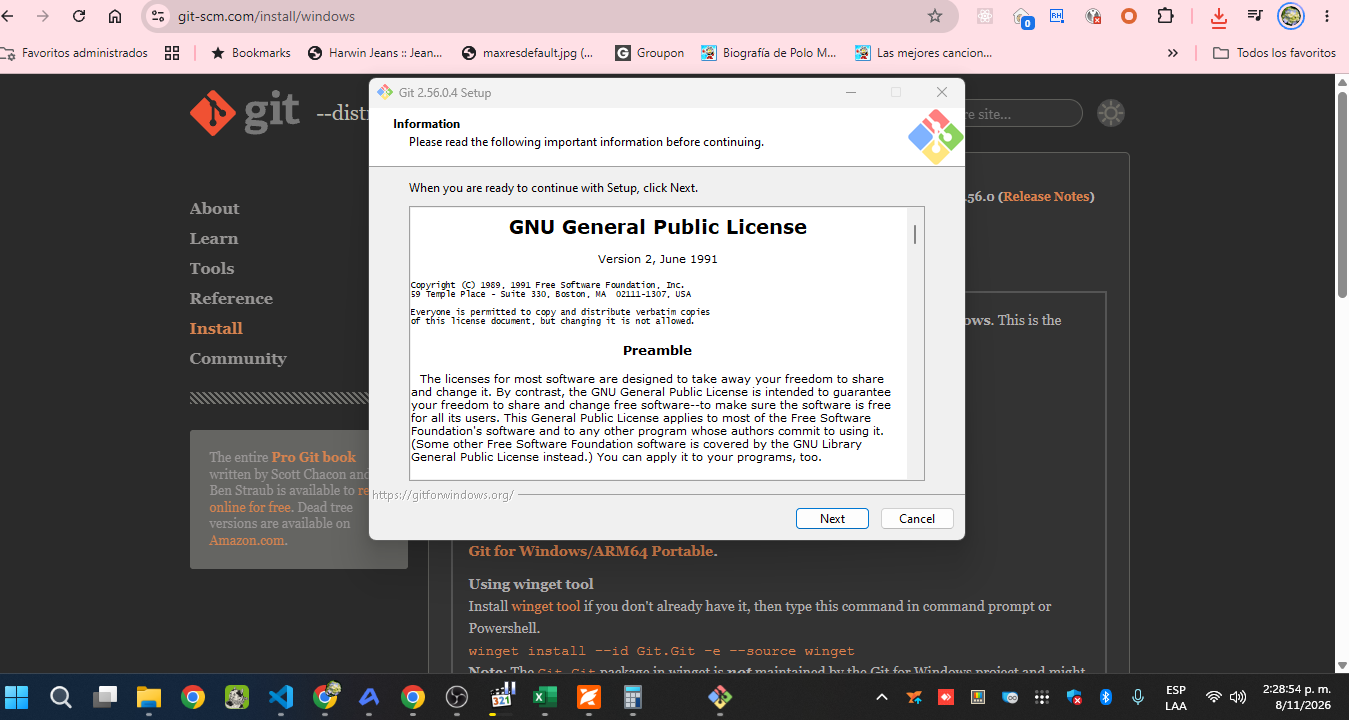
\includegraphics[width=0.85\linewidth]{images/local/paso_03.png}
    \caption{Selección de la carpeta de destino en el disco del sistema.}
    \label{fig:local_03}
\end{figure}

\subsection{Paso 4: Selección de Componentes de la Instalación}
Se activan las casillas clave: \textit{Windows Explorer Integration} (\texttt{Git Bash Here} y \texttt{Git GUI Here}), soporte de archivos grandes (\textit{Git LFS}) y asociación de archivos de configuración \texttt{.git*} y scripts \texttt{.sh}.

\begin{figure}[H]
    \centering
    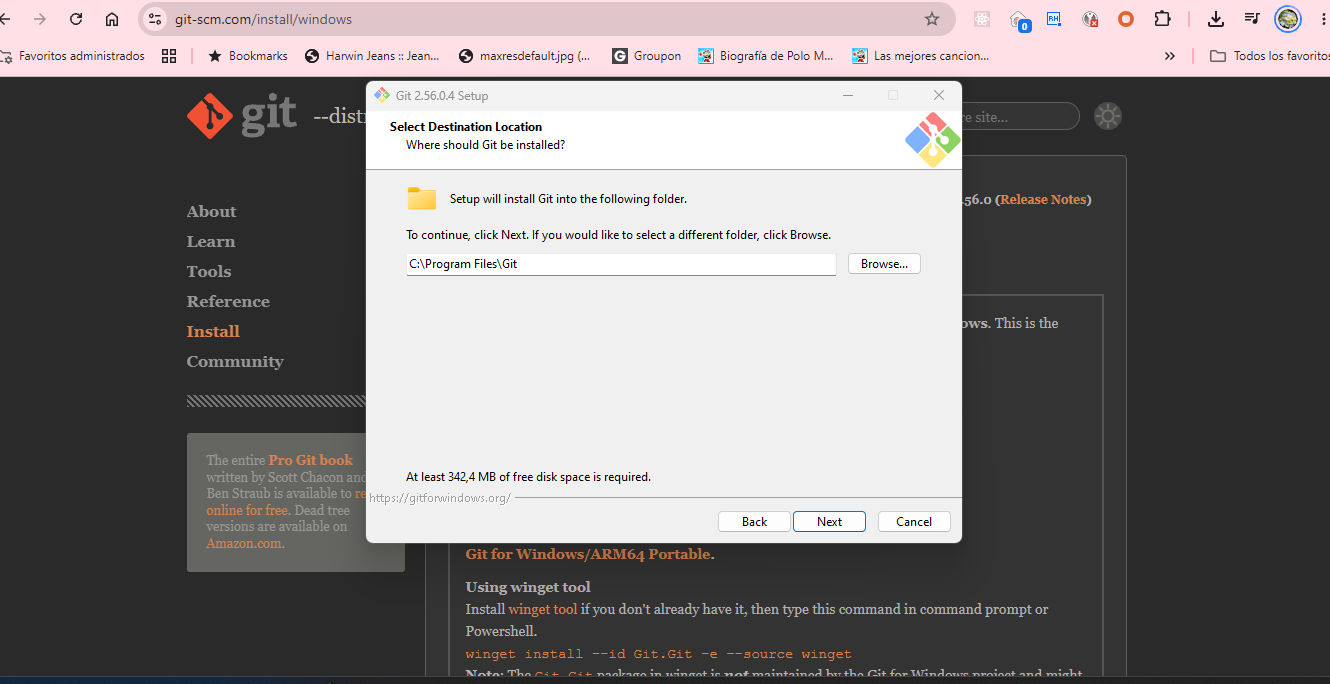
\includegraphics[width=0.85\linewidth]{images/local/paso_04.png}
    \caption{Selección de componentes de integración con el Explorador de Windows y Git LFS.}
    \label{fig:local_04}
\end{figure}

\newpage

\subsection{Paso 5: Configuración de la Carpeta del Menú Inicio}
Se define el nombre del grupo de accesos directos en el menú de inicio como \texttt{Git}.

\begin{figure}[H]
    \centering
    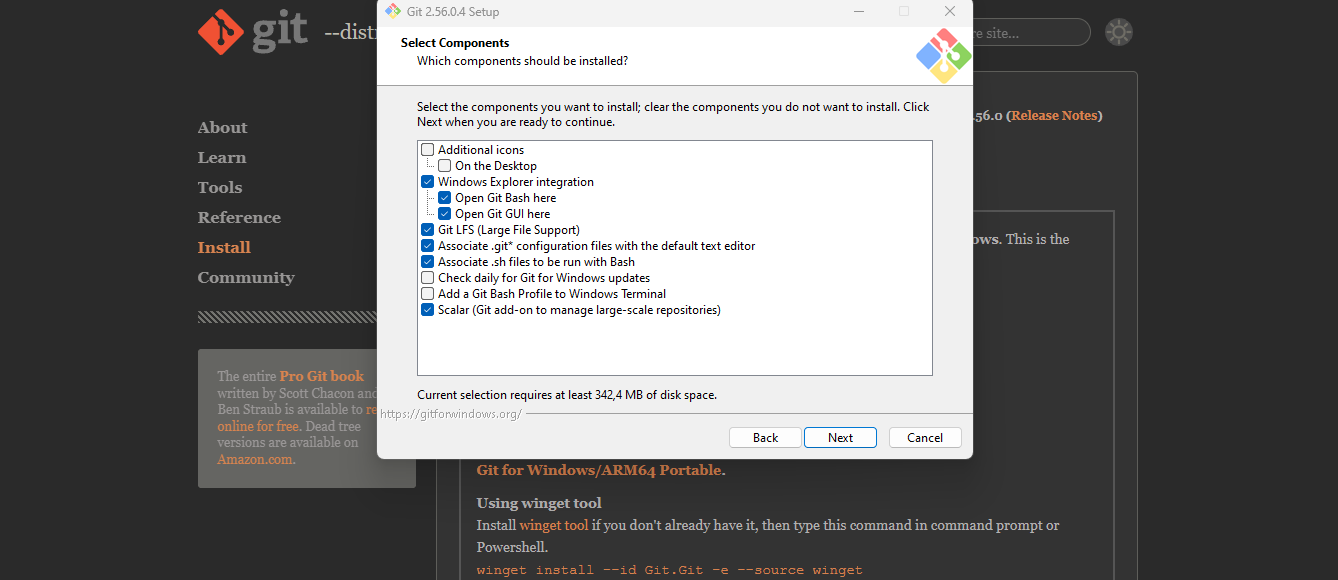
\includegraphics[width=0.85\linewidth]{images/local/paso_05.png}
    \caption{Configuración del acceso directo en el Menú Inicio de Windows.}
    \label{fig:local_05}
\end{figure}

\subsection{Paso 7: Selección del Editor de Texto Predeterminado}
Se selecciona el editor que Git abrirá automáticamente al solicitar mensajes interactivos de confirmación o resolución de conflictos (Vim, Notepad++ o Visual Studio Code).

\begin{figure}[H]
    \centering
    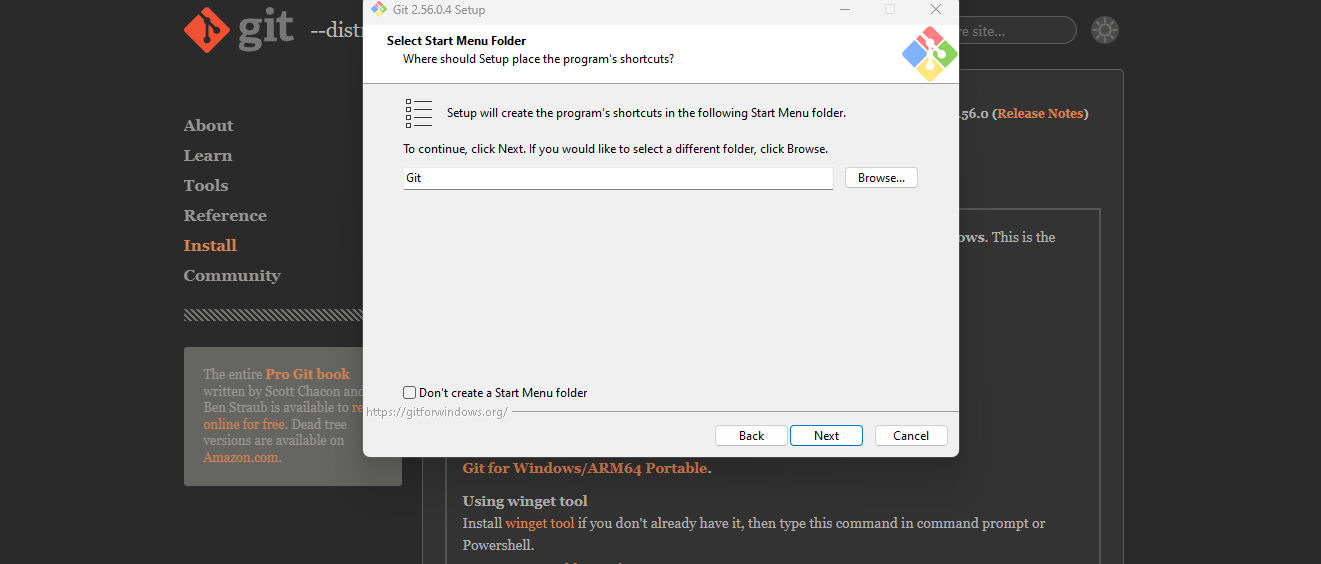
\includegraphics[width=0.85\linewidth]{images/local/paso_07.png}
    \caption{Selección del editor de texto por defecto para operaciones interactivas.}
    \label{fig:local_07}
\end{figure}

\newpage

\subsection{Paso 8: Ajuste del Nombre de la Rama Inicial en Nuevos Repositorios}
Se configura el nombre de la rama por defecto al inicializar repositorios con \texttt{git init}. Se selecciona la directiva moderna \textbf{Override the default branch name} con el valor \texttt{main}, alineado con los estándares internacionales de la industria y GitHub.

\begin{figure}[H]
    \centering
    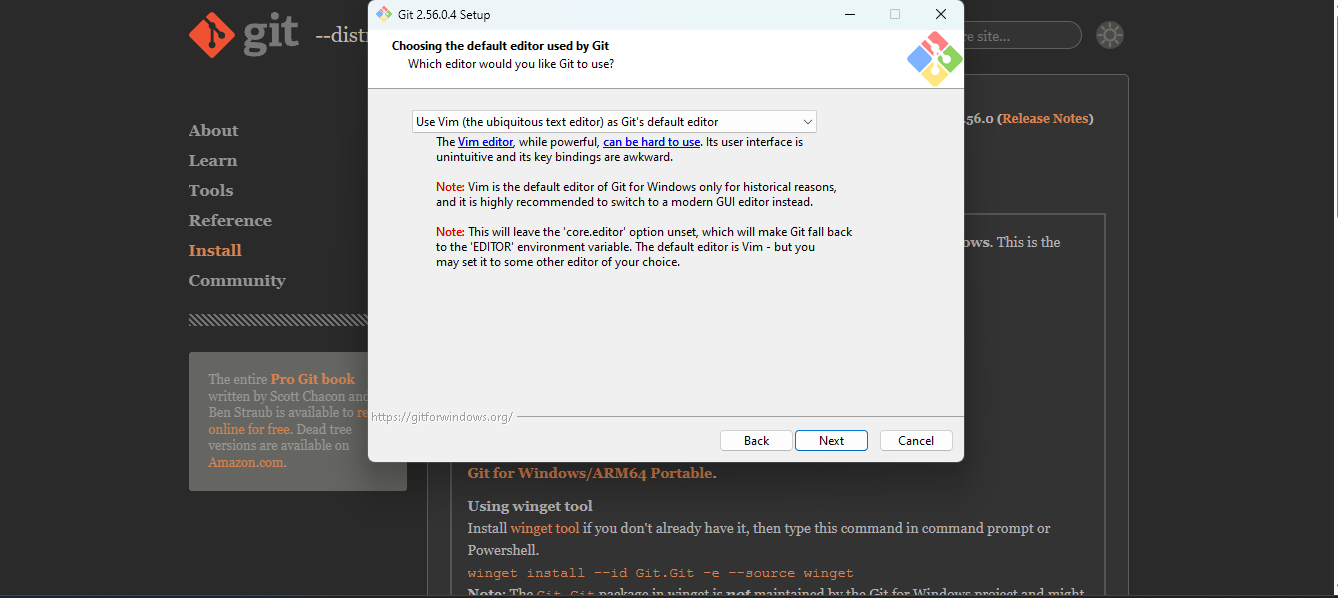
\includegraphics[width=0.85\linewidth]{images/local/paso_08.png}
    \caption{Configuración del nombre de la rama principal inicial como \texttt{main}.}
    \label{fig:local_08}
\end{figure}

\subsection{Paso 9: Ajuste del Entorno PATH}
Se selecciona la opción recomendada: \textbf{Git from the command line and also from 3rd-party software}. Esta alternativa añade los ejecutables mínimos de Git a las variables de entorno de Windows, permitiendo utilizar comandos tanto desde \textit{Git Bash} como desde el \textit{Símbolo del Sistema (CMD)}, PowerShell y la terminal integrada de VS Code.

\begin{figure}[H]
    \centering
    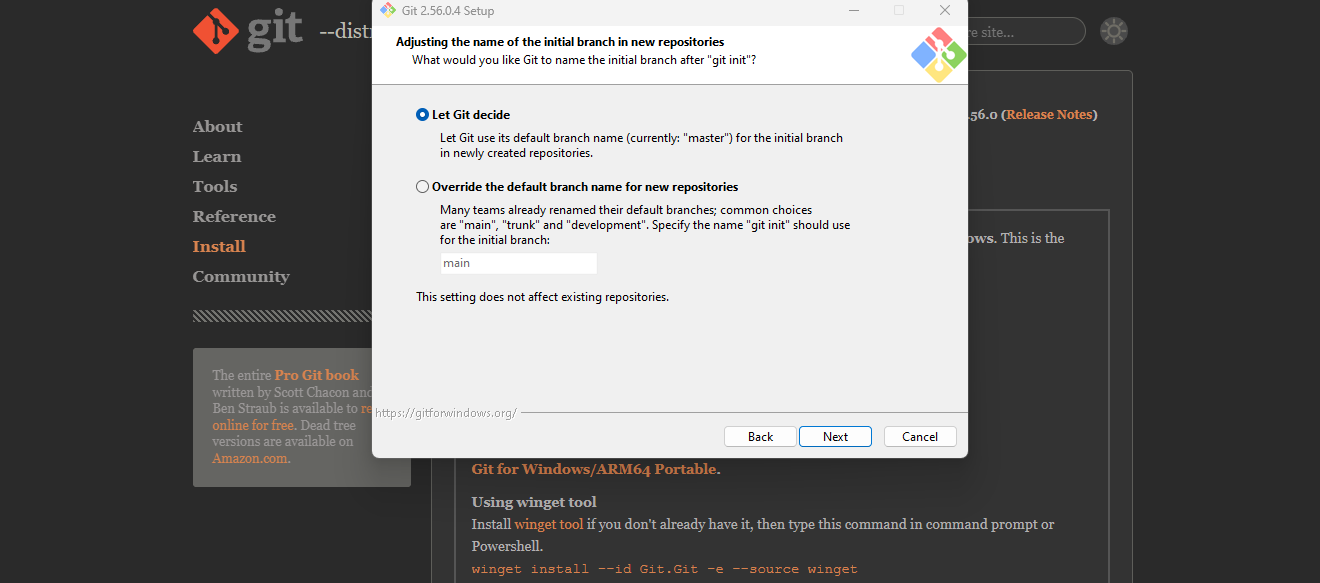
\includegraphics[width=0.85\linewidth]{images/local/paso_09.png}
    \caption{Ajuste de las variables de entorno PATH para compatibilidad con terminales.}
    \label{fig:local_09}
\end{figure}

\newpage

\subsection{Paso 10: Selección del Cliente SSH}
Se elige \textbf{Use bundled OpenSSH}, utilizando el paquete seguro y actualizado de OpenSSH incluido directamente en el instalador de Git.

\begin{figure}[H]
    \centering
    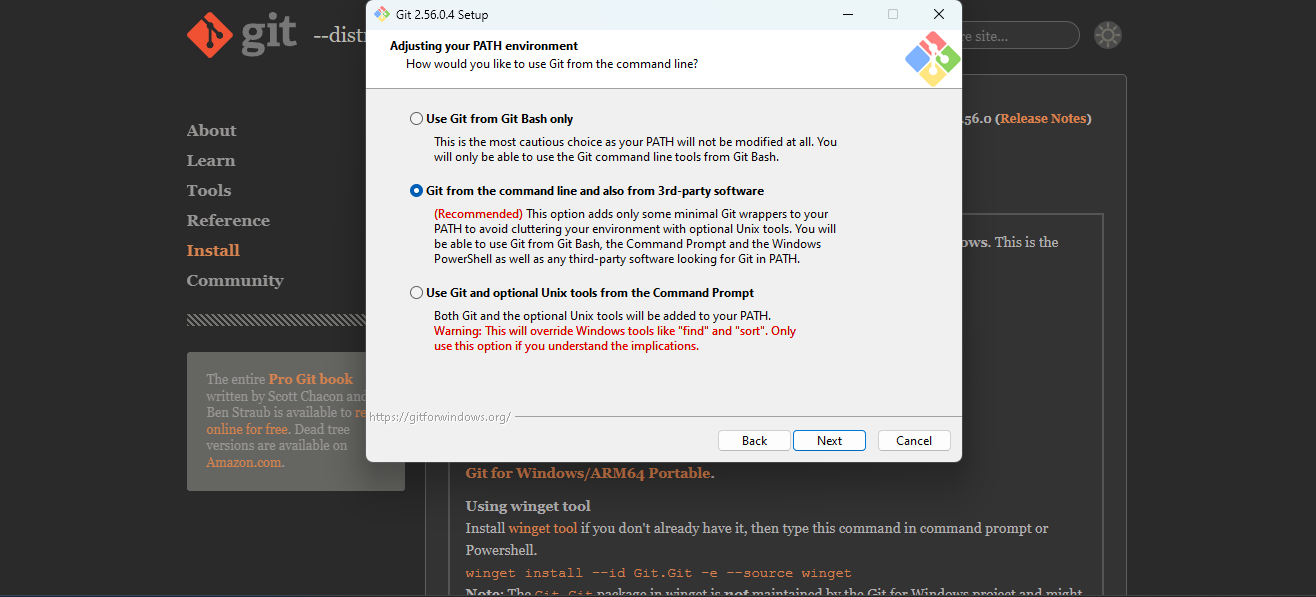
\includegraphics[width=0.85\linewidth]{images/local/paso_10.png}
    \caption{Elección del ejecutable SSH OpenSSH integrado.}
    \label{fig:local_10}
\end{figure}

\subsection{Paso 11: Selección del Backend de Transporte HTTPS}
Se selecciona \textbf{Use the OpenSSL library}, garantizando la validación de certificados criptográficos mediante el almacén estándar \texttt{ca-bundle.crt}.

\begin{figure}[H]
    \centering
    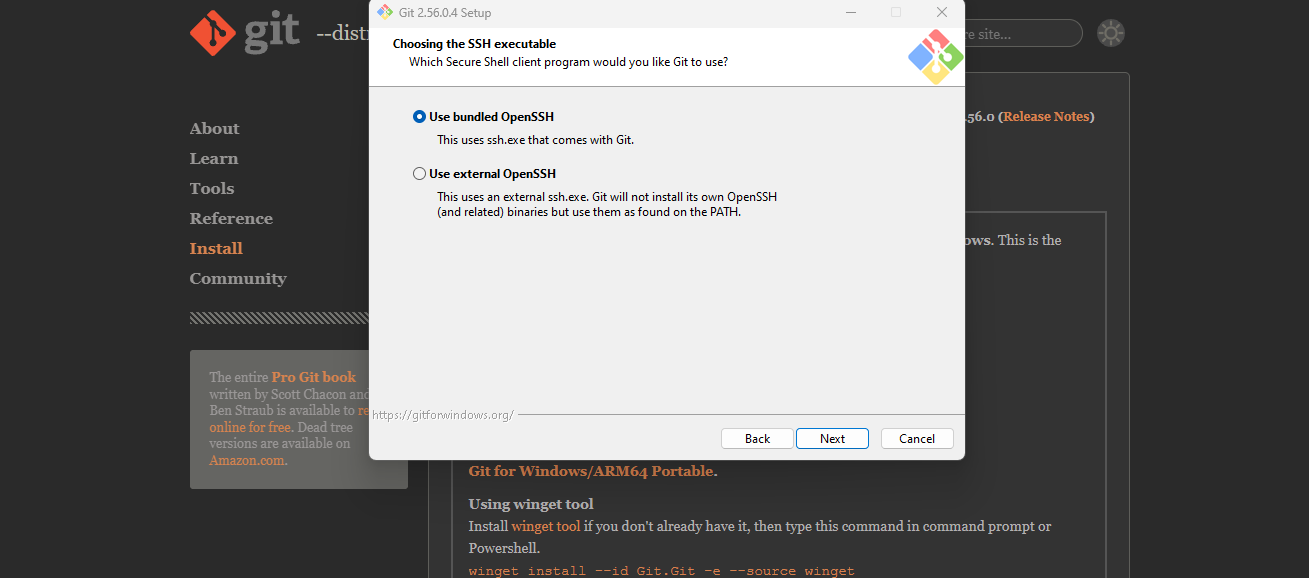
\includegraphics[width=0.85\linewidth]{images/local/paso_11.png}
    \caption{Selección de la biblioteca OpenSSL para conexiones HTTPS seguras.}
    \label{fig:local_11}
\end{figure}

\newpage

\subsection{Paso 12: Configuración de la Conversión de Finales de Línea}
Se elige la directiva recomendada para sistemas Windows: \textbf{Checkout Windows-style, commit Unix-style line endings} (\texttt{core.autocrlf = true}). Esto garantiza que al descargar archivos se conviertan a CRLF para Windows, pero al confirmar hacia el repositorio remoto se normalicen como LF (Unix), previniendo conflictos entre desarrolladores de distintos sistemas operativos.

\begin{figure}[H]
    \centering
    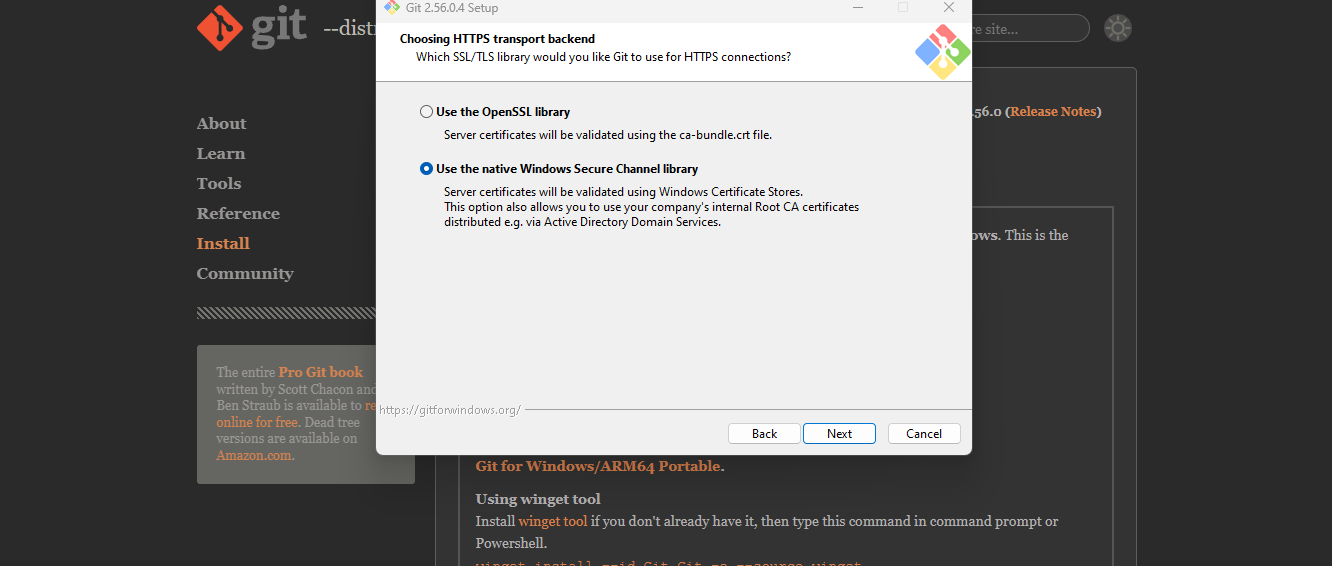
\includegraphics[width=0.85\linewidth]{images/local/paso_12.png}
    \caption{Normalización de finales de línea CRLF/LF con \texttt{core.autocrlf}.}
    \label{fig:local_12}
\end{figure}

\subsection{Paso 13: Configuración del Emulador de Terminal para Git Bash}
Se selecciona \textbf{Use MinTTY (the default terminal of MSYS2)}, proporcionando una consola moderna con soporte UTF-8, redimensionamiento dinámico y tipografía nítida.

\begin{figure}[H]
    \centering
    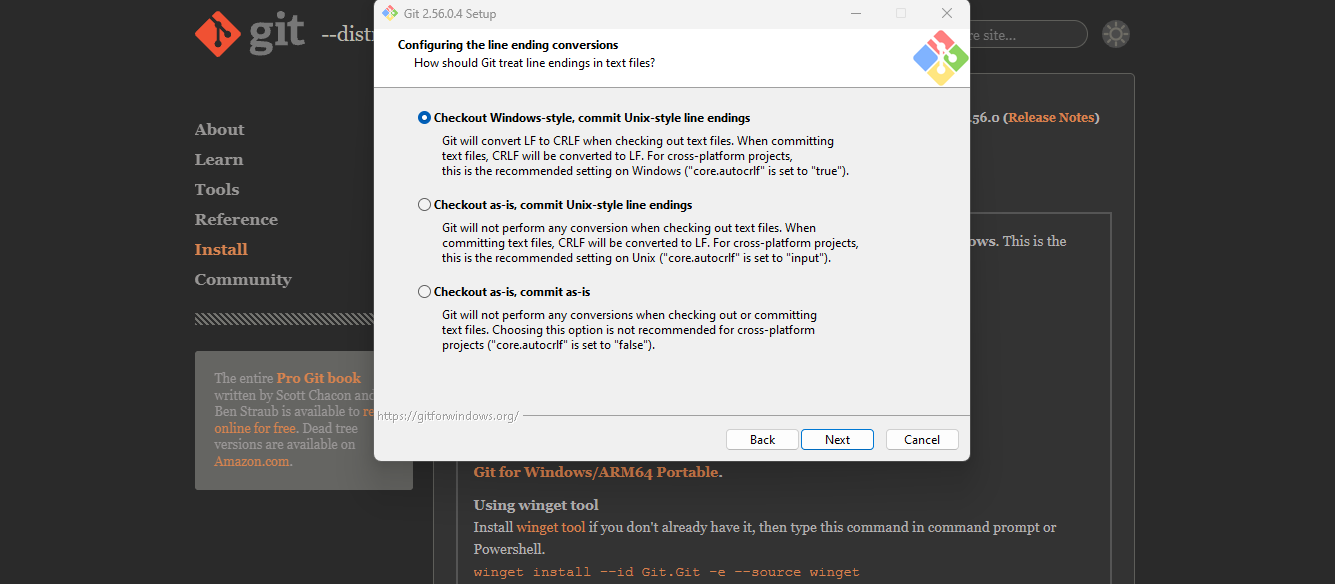
\includegraphics[width=0.85\linewidth]{images/local/paso_13.png}
    \caption{Configuración del emulador de terminal MinTTY para Git Bash.}
    \label{fig:local_13}
\end{figure}

\newpage

\subsection{Paso 14: Comportamiento Predeterminado de \texttt{git pull}}
Se selecciona \textbf{Default (fast-forward or merge)}, asegurando que al sincronizar cambios se aplique avance rápido si es posible, o se genere un commit de fusión estándar.

\begin{figure}[H]
    \centering
    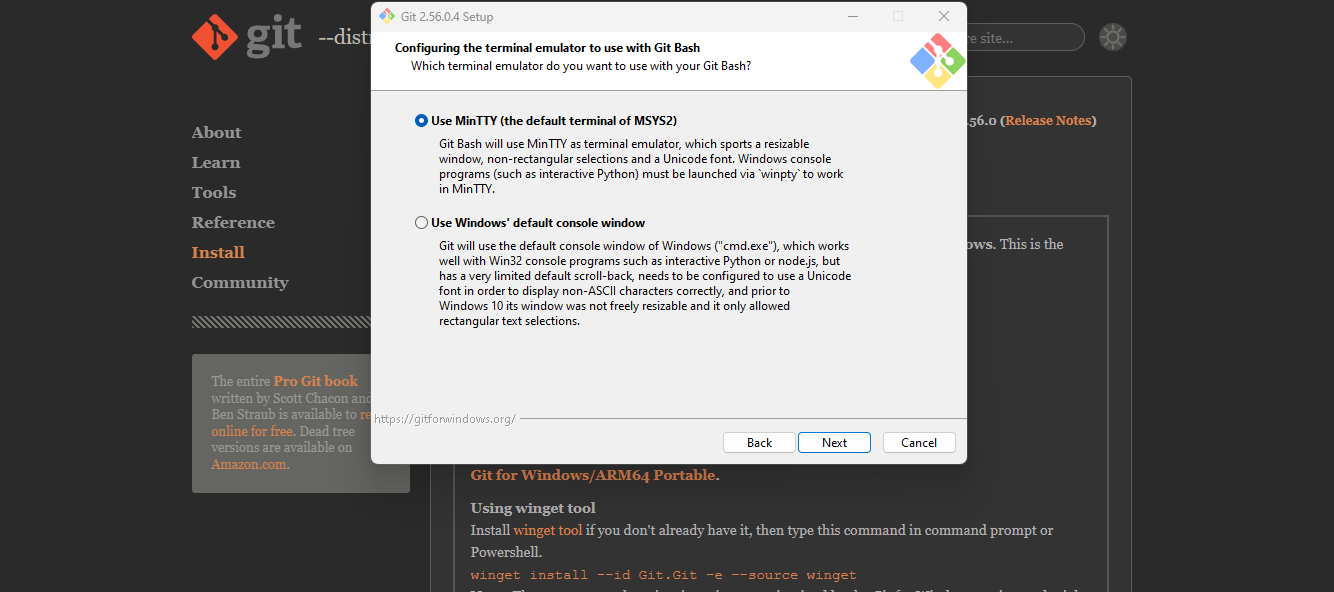
\includegraphics[width=0.85\linewidth]{images/local/paso_14.png}
    \caption{Comportamiento de integración para el comando \texttt{git pull}.}
    \label{fig:local_14}
\end{figure}

\subsection{Paso 15: Selección del Asistente de Credenciales}
Se activa \textbf{Git Credential Manager (GCM)}, el cual administra de forma transparente y cifrada los tokens de acceso personal y autenticación multifactor (2FA) con GitHub en el Administrador de Credenciales de Windows.

\begin{figure}[H]
    \centering
    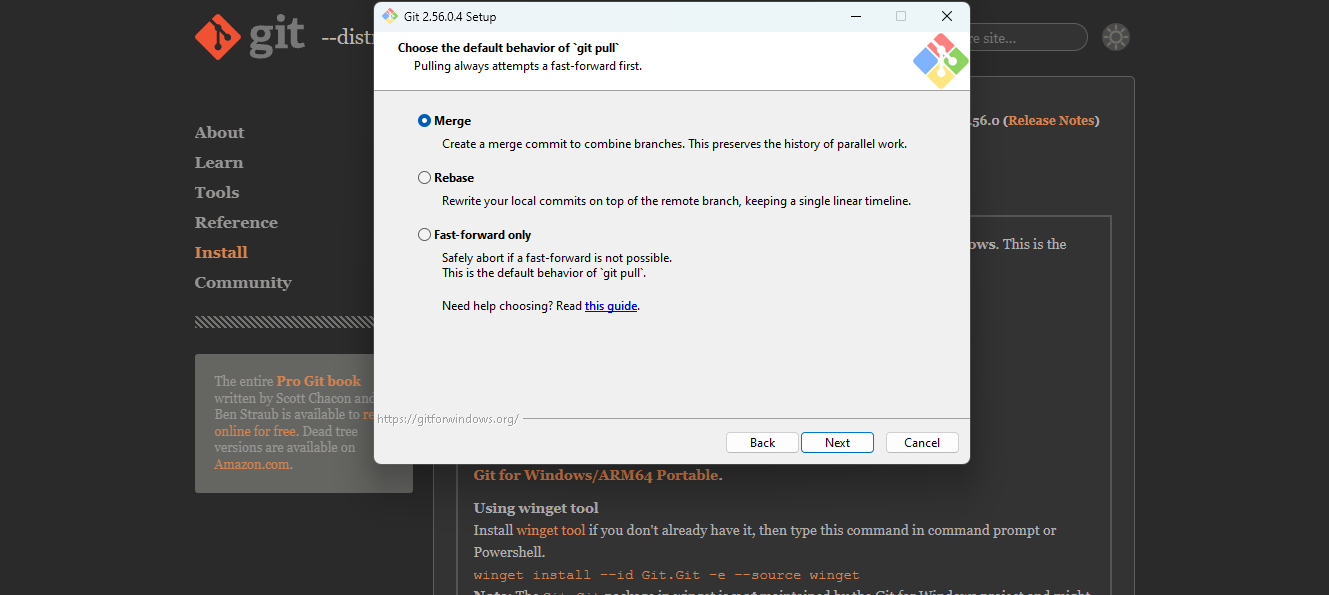
\includegraphics[width=0.85\linewidth]{images/local/paso_15.png}
    \caption{Habilitación de Git Credential Manager para autenticación segura.}
    \label{fig:local_15}
\end{figure}

\newpage

\subsection{Paso 16: Configuración de Opciones de Rendimiento y Caché}
Se activa \textbf{Enable file system caching}, permitiendo almacenar en memoria metadatos de archivos para acelerar de manera notable operaciones como \texttt{git status} y \texttt{git diff} en repositorios grandes.

\begin{figure}[H]
    \centering
    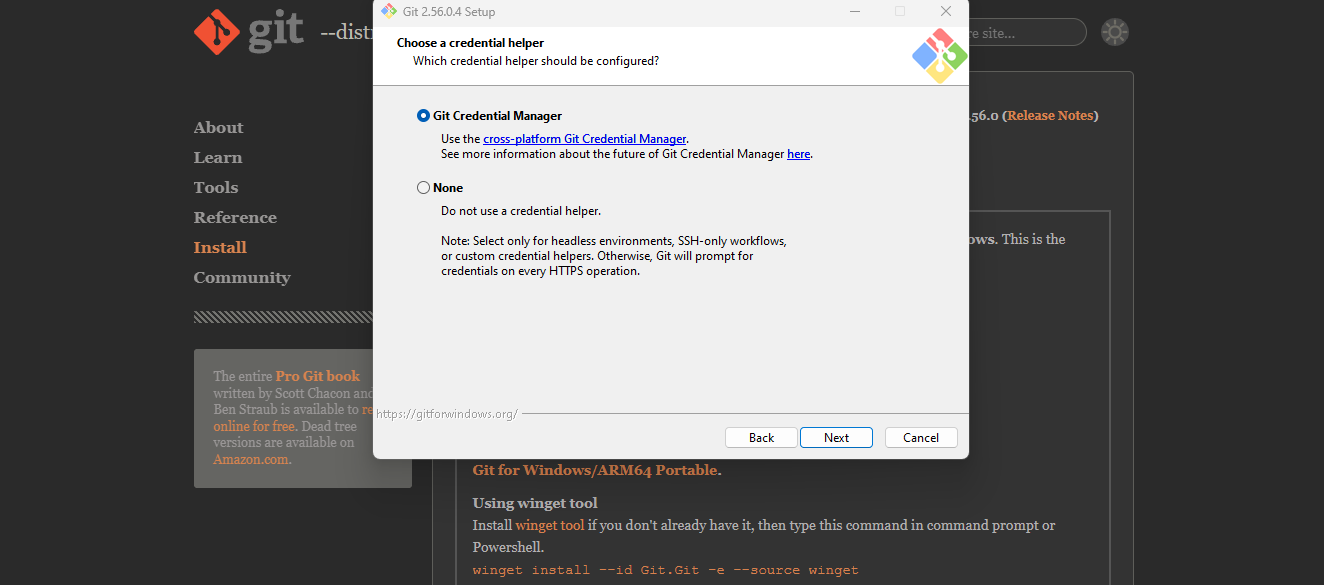
\includegraphics[width=0.85\linewidth]{images/local/paso_16.png}
    \caption{Habilitación del caché del sistema de archivos para máxima velocidad.}
    \label{fig:local_16}
}
\end{figure}

\subsection{Paso 17: Opciones Experimentales}
Se mantienen desmarcadas las opciones experimentales para garantizar máxima estabilidad en el entorno productivo de la aprendiz.

\begin{figure}[H]
    \centering
    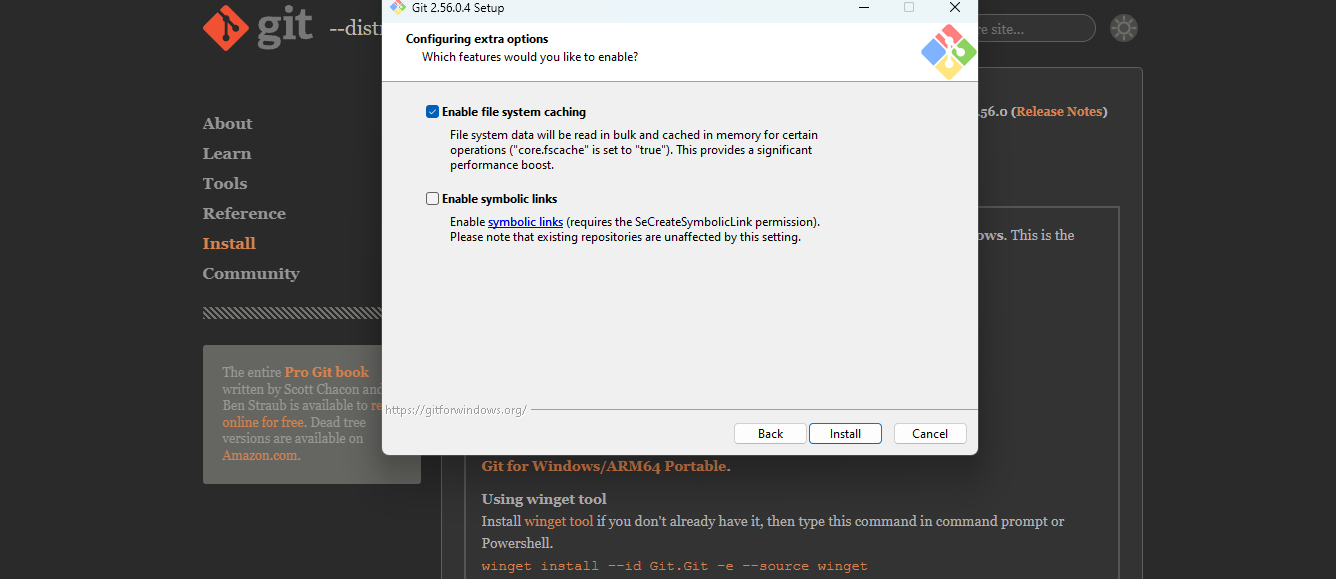
\includegraphics[width=0.85\linewidth]{images/local/paso_17.png}
    \caption{Panel de opciones experimentales mantenidas en modo seguro.}
    \label{fig:local_17}
\end{figure}

\newpage

\subsection{Paso 18: Proceso de Instalación y Extracción de Archivos}
El asistente descomprime las librerías, herramientas CLI y emuladores en la ruta de destino.

\begin{figure}[H]
    \centering
    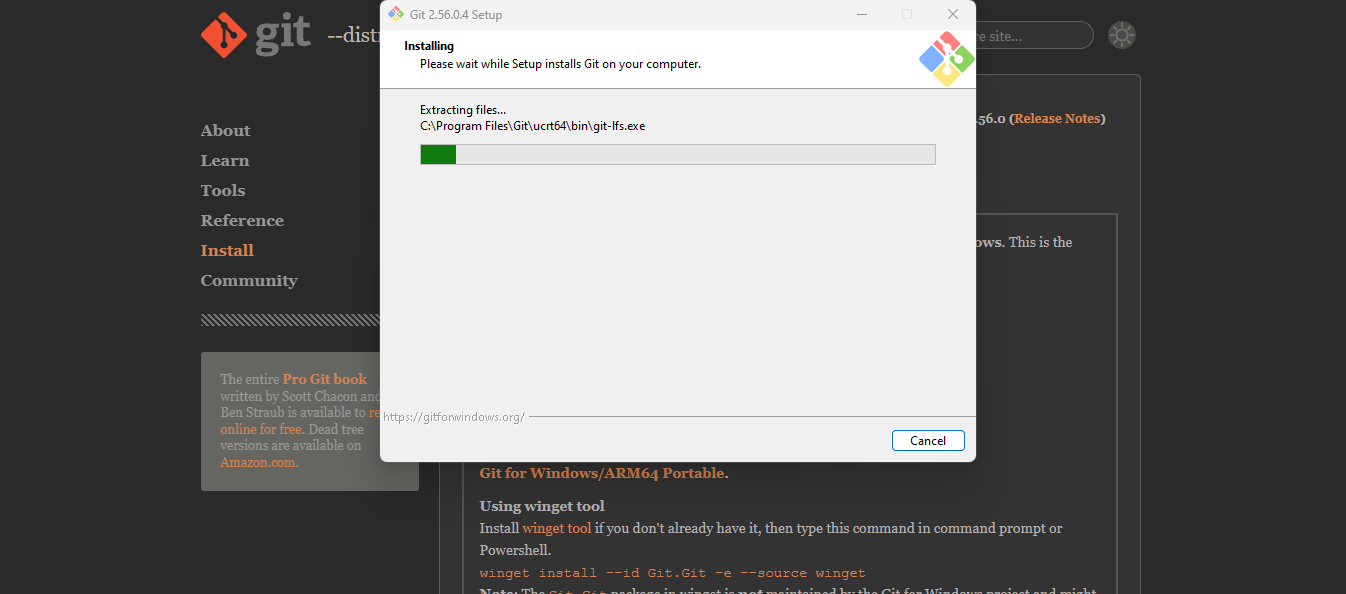
\includegraphics[width=0.85\linewidth]{images/local/paso_18.png}
    \caption{Extracción e instalación de paquetes binarios de Git.}
    \label{fig:local_18}
\end{figure}

\subsection{Paso 19: Finalización Exitosa del Asistente de Instalación}
Se concluye la instalación con la opción de lanzar inmediatamente \textit{Git Bash}.

\begin{figure}[H]
    \centering
    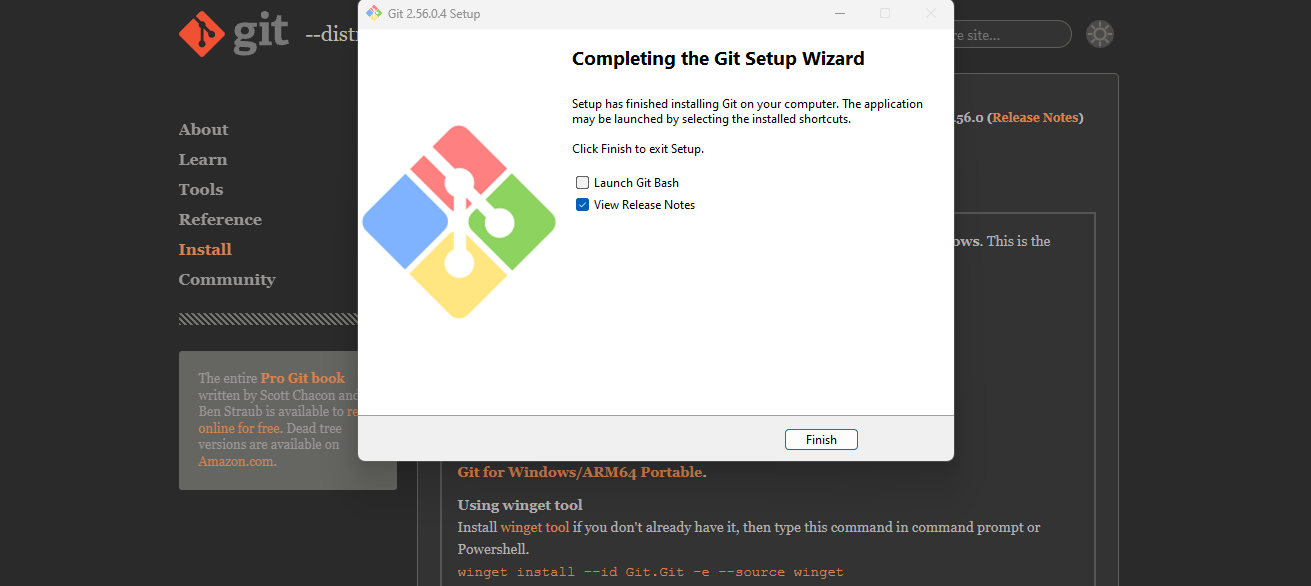
\includegraphics[width=0.85\linewidth]{images/local/paso_19.png}
    \caption{Finalización exitosa del asistente de instalación de Git para Windows.}
    \label{fig:local_19}
\end{figure}

\newpage

\subsection{Paso 20: Verificación de Versión y Parametrización en Consola}
En la consola de comandos se valida la correcta instalación de Git y se registran las credenciales globales de identidad de la aprendiz Karen Yuliana Campo:

\begin{figure}[H]
    \centering
    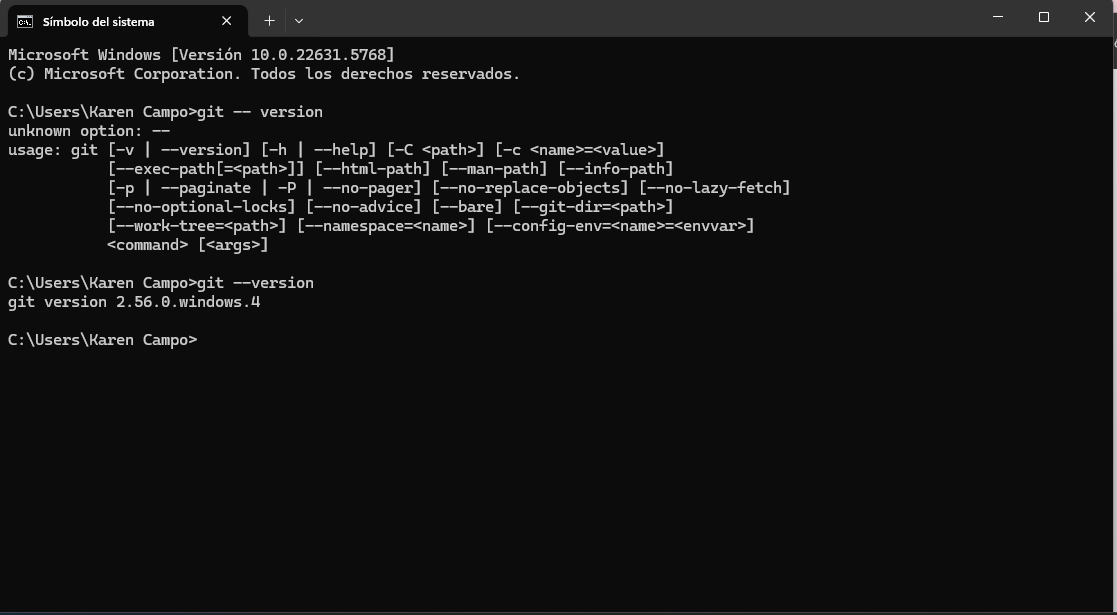
\includegraphics[width=0.85\linewidth]{images/local/paso_20.png}
    \caption{Verificación de versión y configuración de identidad en Git Bash / Terminal.}
    \label{fig:local_20}
\end{figure}

\begin{cmdbox}
\textbf{\color{white}Comandos ejecutados para la verificación e identidad:}
\begin{lstlisting}[language=bash]
# 1. Comprobacion de la version instalada
git --version
# Salida esperada: git version 2.xx.x.windows.1

# 2. Configuracion del nombre formal de la aprendiz
git config --global user.name "Karen Yuliana Campo"

# 3. Configuracion del correo institucional/personal
git config --global user.email "karen.campo@sena.edu.co"

# 4. Establecer main como rama predeterminada global
git config --global init.defaultBranch main

# 5. Auditoria de la configuracion aplicada
git config --list --show-origin
\end{lstlisting}
\end{cmdbox}

\newpage

% =========================================================================
% SECCIÓN 4: REGISTRO Y CONFIGURACIÓN DE GIT REMOTO (GITHUB)
% =========================================================================
\section{Configuración de Cuenta Remota en GitHub (Paso a Paso con Capturas Reales)}

Para habilitar la sincronización en la nube, respaldo y trabajo colaborativo, se efectuó el proceso de registro en la plataforma oficial de GitHub:

\subsection{Paso 1: Acceso al Portal Oficial de GitHub}
Se ingresa a \url{https://github.com/} y se selecciona la opción \textbf{Sign up} en la esquina superior derecha para iniciar el asistente interactivo de registro.

\begin{figure}[H]
    \centering
    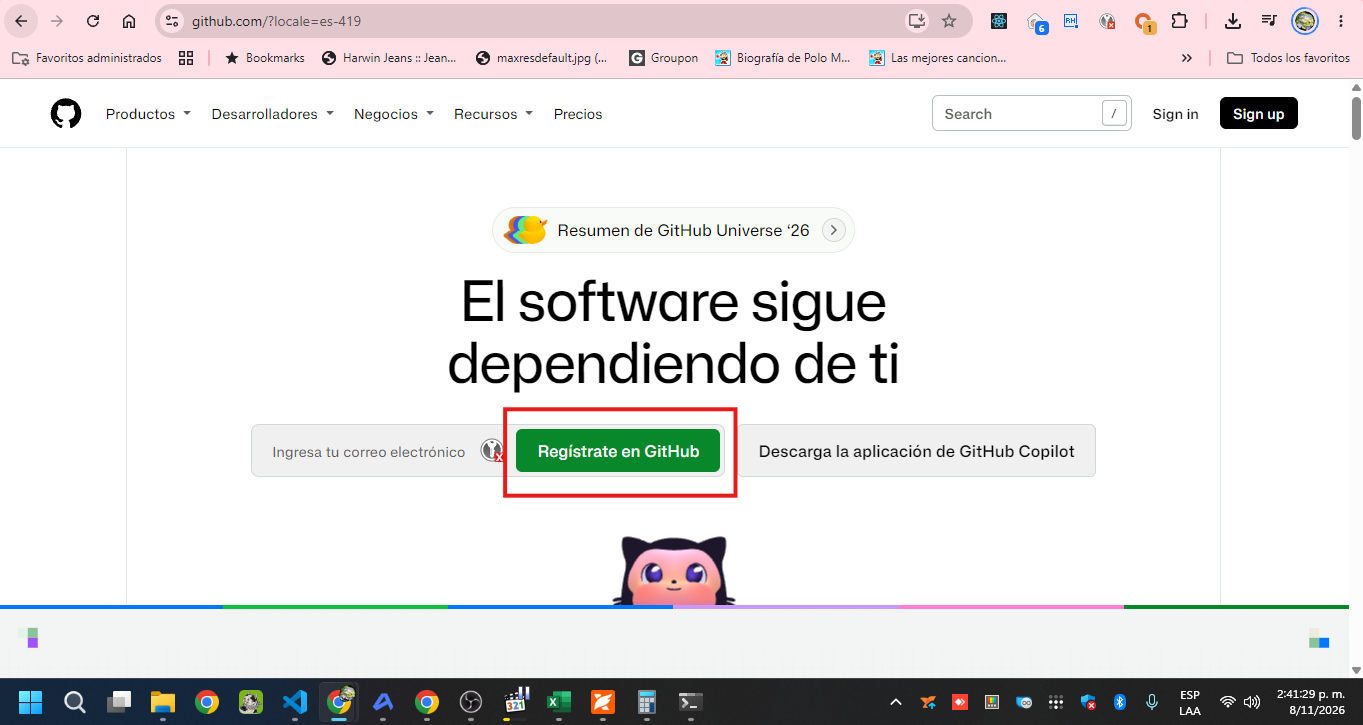
\includegraphics[width=0.88\linewidth]{images/remoto/paso_01.png}
    \caption{Pantalla principal de GitHub y acceso al registro de usuario.}
    \label{fig:remoto_01}
\end{figure}

\subsection{Paso 2: Registro de Correo Electrónico}
Se ingresa el correo electrónico personal/institucional que servirá como identificador único de la cuenta y receptor de notificaciones.

\begin{figure}[H]
    \centering
    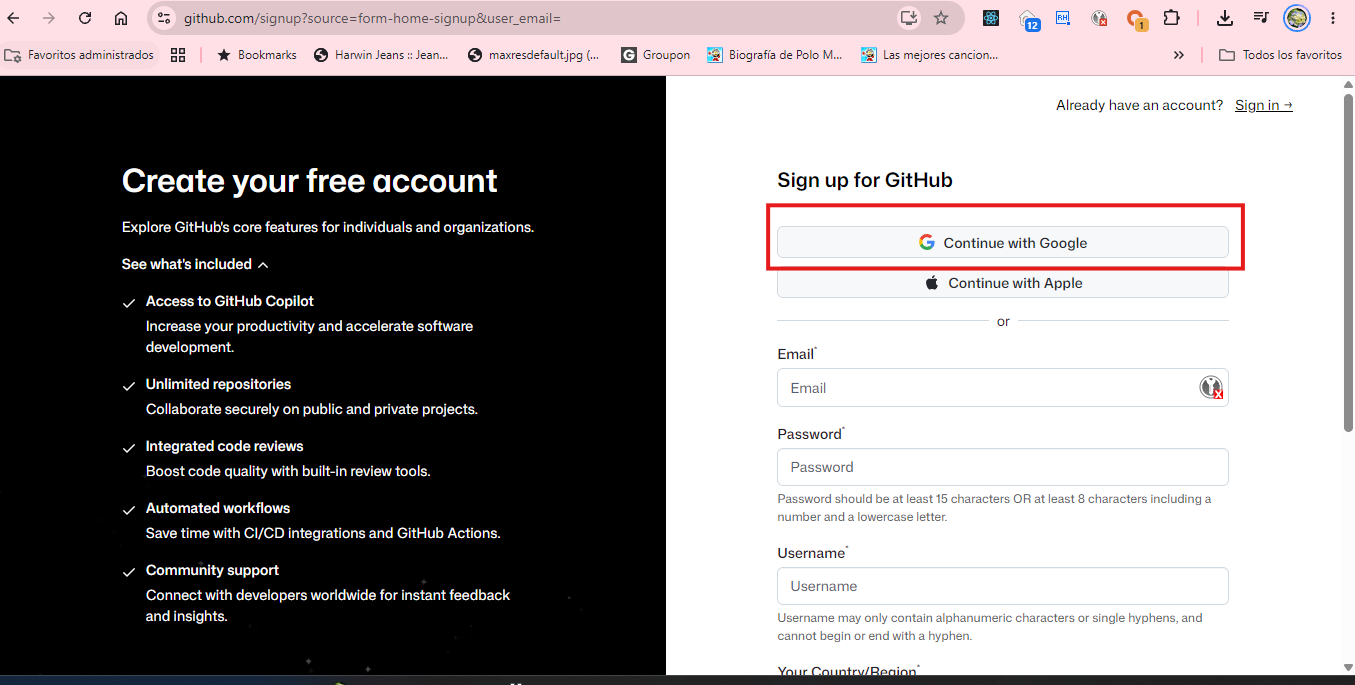
\includegraphics[width=0.85\linewidth]{images/remoto/paso_02.png}
    \caption{Ingreso del correo electrónico de registro en GitHub.}
    \label{fig:remoto_02}
\end{figure}

\newpage

\subsection{Paso 3: Creación de Contraseña y Selección de Nombre de Usuario}
Se define una contraseña de alta seguridad ($>15$ caracteres con combinación alfanumérica y caracteres especiales) y se elige el nombre de usuario de la aprendiz (\textit{username}) para el perfil público.

\begin{figure}[H]
    \centering
    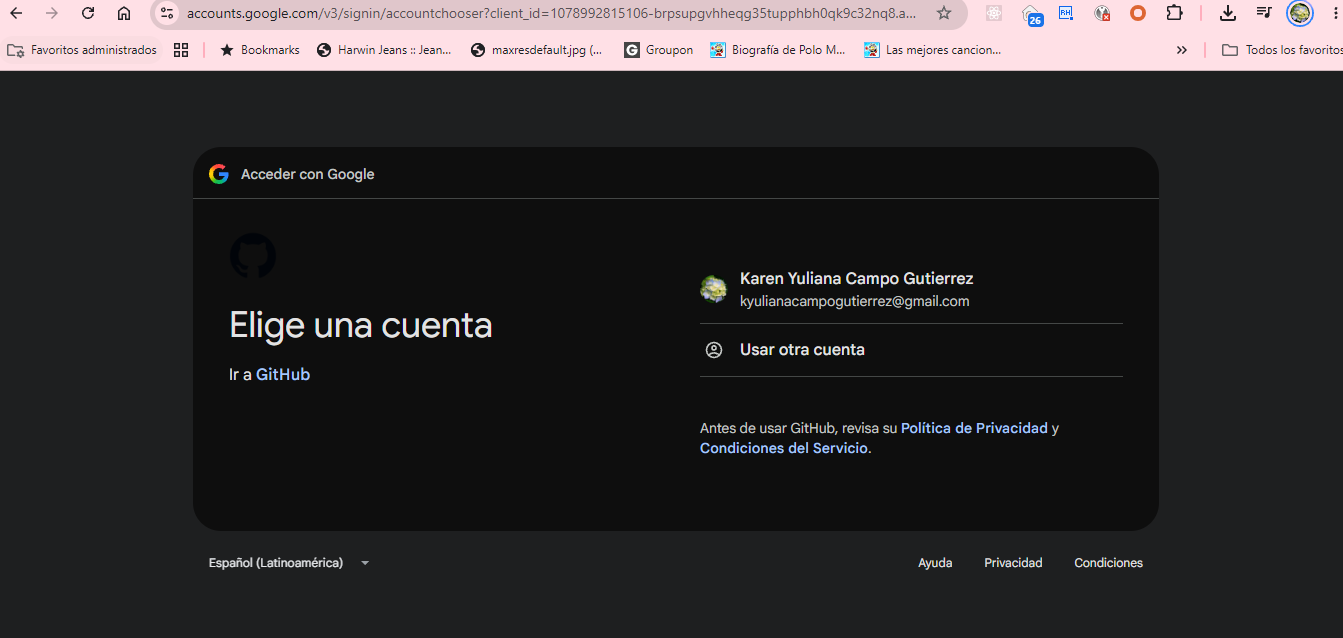
\includegraphics[width=0.85\linewidth]{images/remoto/paso_03.png}
    \caption{Definición de credenciales de acceso y nombre de usuario.}
    \label{fig:remoto_03}
\end{figure}

\subsection{Paso 4: Verificación de Seguridad (Puzzle Humano)}
Se resuelve el reto de seguridad interactivo para demostrar autenticidad humana y prevenir la creación automatizada de cuentas no autorizadas.

\begin{figure}[H]
    \centering
    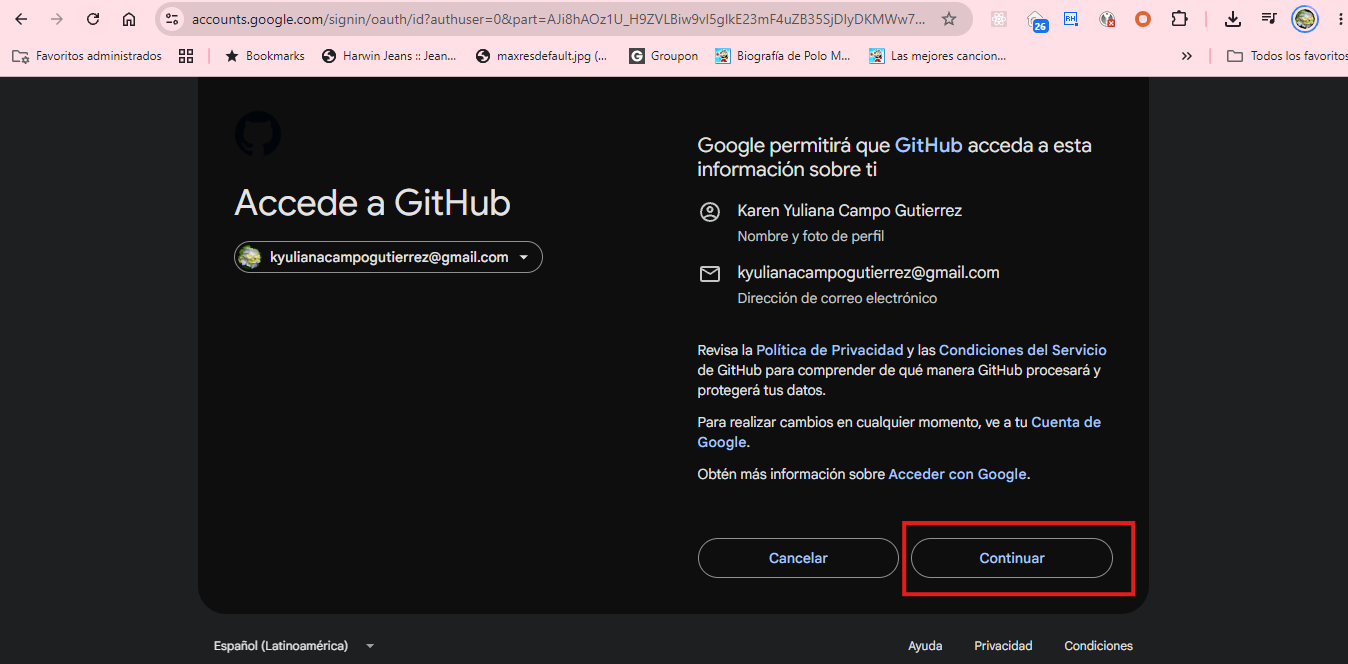
\includegraphics[width=0.85\linewidth]{images/remoto/paso_04.png}
    \caption{Resolución del acertijo de verificación humana de GitHub.}
    \label{fig:remoto_04}
\end{figure}

\newpage

\subsection{Paso 5: Validación del Código de Correo y Acceso al Dashboard}
Se ingresa el código numérico de 8 dígitos enviado por GitHub al correo electrónico de la aprendiz, desbloqueando el acceso inmediato al panel principal (\textit{Dashboard}) de bienvenida en GitHub.

\begin{figure}[H]
    \centering
    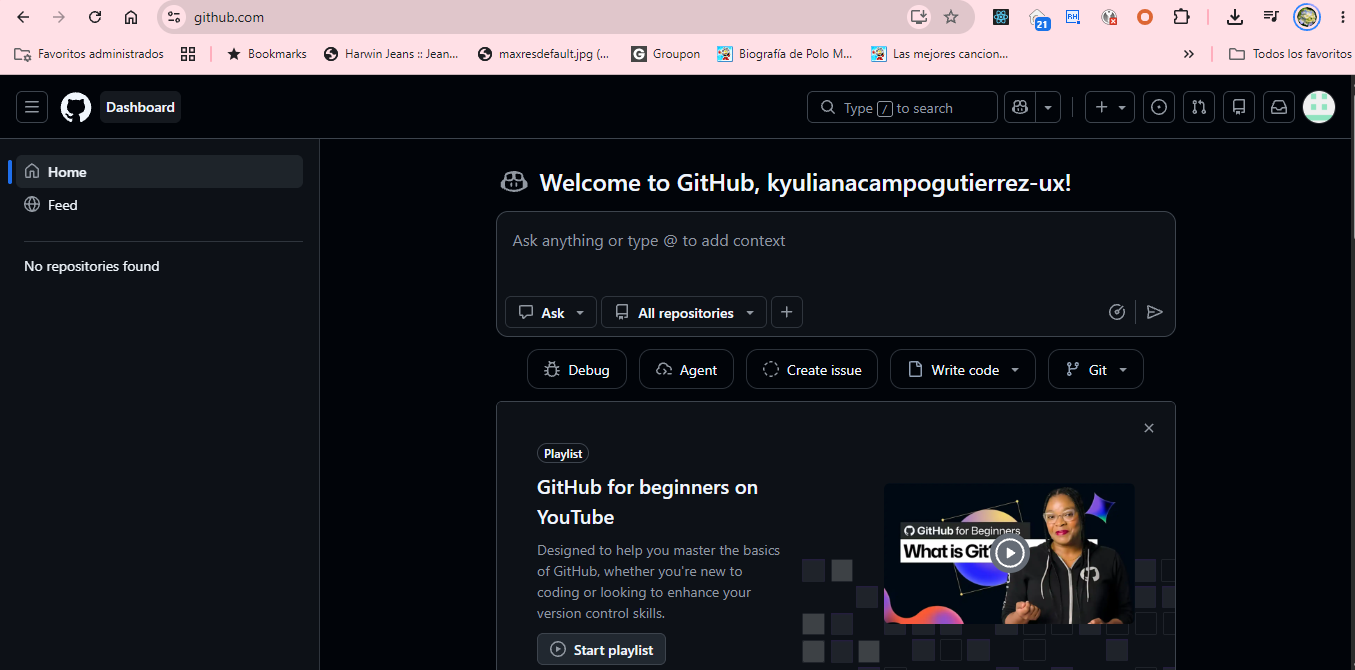
\includegraphics[width=0.88\linewidth]{images/remoto/paso_05.png}
    \caption{Ingreso del código de confirmación y bienvenida al dashboard de GitHub.}
    \label{fig:remoto_05}
\end{figure}

% =========================================================================
% SECCIÓN 5: VINCULACIÓN ENTRE GIT LOCAL Y GITHUB
% =========================================================================
\section{Vinculación Operativa entre el Equipo Local y el Repositorio Remoto}

Con ambas herramientas instaladas y configuradas, el puente de conexión se formaliza mediante los siguientes pasos técnicos en la terminal:

\begin{cmdbox}
\textbf{\color{white}Flujo de vinculacion del proyecto Pizzería Bella Italia:}
\begin{lstlisting}[language=bash]
# 1. Posicionarse en el directorio del proyecto (en Git Bash)
cd ~/Desktop/SENA/CDE

# 2. Inicializar repositorio local si es un proyecto nuevo
git init -b main

# 3. Vincular el repositorio remoto de GitHub con el alias origin
git remote add origin https://github.com/karen-campo/pizzeria-bella-italia.git

# 4. Verificar la conexion remota configurada
git remote -v
# origin  https://github.com/karen-campo/pizzeria-bella-italia.git (fetch)
# origin  https://github.com/karen-campo/pizzeria-bella-italia.git (push)

# 5. Preparar y confirmar los archivos iniciales
git add .
git commit -m "feat: inicializacion de la arquitectura de software de la pizzeria"

# 6. Publicar la rama main en GitHub con seguimiento ascendente
git push -u origin main
\end{lstlisting}
\end{cmdbox}

\newpage

% =========================================================================
% SECCIÓN 6: RÚBRICA SENA
% =========================================================================
\section{Matriz de Cumplimiento de la Lista de Chequeo SENA}

Evaluación exhaustiva frente al instrumento \textbf{IE-GA7-220501096-AA1-EV04}:

\begin{table}[H]
\centering
\small
\begin{tabular}{p{7.5cm}cp{5.5cm}}
\toprule
\textbf{Criterio de Evaluación de la Guía 7} & \textbf{Cumplimiento} & \textbf{Evidencia en el Documento} \\
\midrule
\textbf{Selecciona y configura herramientas de versionamiento para el control de cambios en el código.} & \textbf{\color{senaGreen}100\% CUMPLE} & Instalación de Git v2.xx para Windows y creación del perfil remoto en GitHub. \\
\addlinespace
\textbf{Paso a paso con pantallazos de la instalación de herramientas local y remota.} & \textbf{\color{senaGreen}100\% CUMPLE} & 19 capturas reales de Git local (Figuras \ref{fig:local_01} a \ref{fig:local_20}) y 5 capturas reales de GitHub (Figuras \ref{fig:remoto_01} a \ref{fig:remoto_05}). \\
\addlinespace
\textbf{Aplica normas básicas de presentación de documentos escritos.} & \textbf{\color{senaGreen}100\% CUMPLE} & Portada formal, introducción, objetivos, metadatos de Karen Yuliana Campo, Popayán, Cauca, Ficha 228118, conclusiones y referencias. \\
\bottomrule
\end{tabular}
\caption{Matriz de evaluación del instrumento IE-GA7-220501096-AA1-EV04.}
\end{table}

% =========================================================================
% SECCIÓN 7: CONCLUSIONES
% =========================================================================
\section{Conclusiones}
\begin{enumerate}[label=\arabic*.]
    \item \textbf{Estandarización desde la instalación:} La selección de parámetros modernos en el asistente de Git (rama por defecto \texttt{main}, integración con PATH y normalización \texttt{core.autocrlf}) previene inconsistencias sintácticas y garantiza que el equipo trabaje bajo estándares de la industria.
    \item \textbf{Seguridad y control de credenciales:} La adopción de \textit{Git Credential Manager} en conjunto con GitHub permite gestionar accesos mediante tokens PAT sin exponer contraseñas en texto plano, cumpliendo con las políticas internacionales de ciberseguridad.
    \item \textbf{Base lista para Integración Continua:} Con el entorno local y remoto plenamente enlazados, el proyecto de la Pizzería Bella Italia cuenta con la plataforma necesaria para desplegar pipelines automatizados de CI/CD con pruebas unitarias TDD.
\end{enumerate}

% =========================================================================
% SECCIÓN 8: REFERENCIAS BIBLIOGRÁFICAS
% =========================================================================
\section{Referencias Bibliográficas}
\begin{itemize}[leftmargin=1.5cm]
    \item Chacon, S., \& Straub, B. (2014). \textit{Pro Git} (2nd ed.). Apress. Recuperado de \url{https://git-scm.com/book/es/v2}
    \item GitHub Docs. (2024). \textit{Setting your commit email address in Git}. Recuperado de \url{https://docs.github.com/en/account-and-profile}
    \item Servicio Nacional de Aprendizaje -- SENA. (2024). \textit{Componente Formativo: Integración continua}. Plataforma Zajuna.
    \item Git for Windows Community. (2024). \textit{Git for Windows v2.xx Release Notes and Architecture}. Recuperado de \url{https://gitforwindows.org}
\end{itemize}

\end{document}
